%%
%% Template LaTeX2e file
%%
\documentclass[a5paper,twoside]{article}
\usepackage{german,color}
\usepackage[utf8]{inputenc}
\usepackage{graphicx}
\usepackage{calc}
\usepackage[linkbordercolor={1 0.7 0.7}]{hyperref}

\hypersetup{
  pdftitle    = {Handbuch Alternativ-Firmware für Sparmatic Comet},
  pdfsubject  = {Alternativ-Firmware für Sparmatic Comet},
  pdfauthor   = {Jörg Wunsch},
  pdfkeywords = {Handbuch},
  pdfcreator  = {pdflatex},
  pdfproducer = {LaTeX with hyperref}
}

\newcommand\SC{"`Sparmatic Comet"'}

\title {
  Bedienungsanleitung Alternativ-Firmware für \SC\\
  \vspace*{1ex}
  {\centering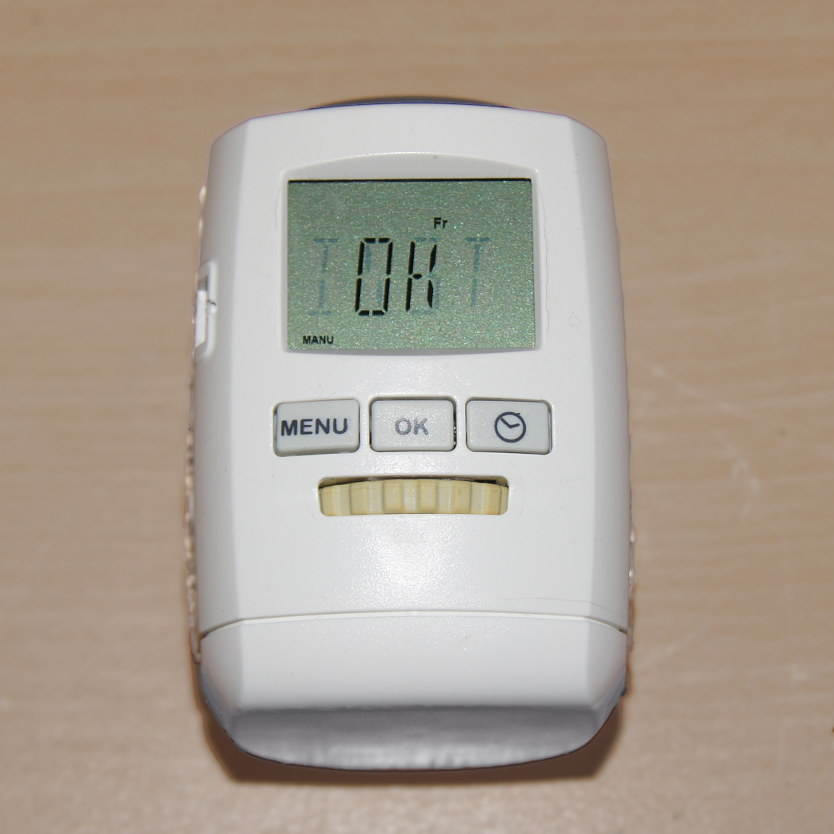
\includegraphics[width=0.63\linewidth]{Comet.jpg}}
}

\author {
Jörg Wunsch
}

%% if you wanna set a specified date:
%\date {
%25-Mar-88
%}

\sloppy

\begin {document}
\maketitle
\thispagestyle{empty}
\pagebreak
\cleardoublepage

\tableofcontents

\section {
Beschreibung der Hardware
}

Die Hardware des \SC{} besteht aus einem Gehäuse, welches auf einen
auf das eigentliche Heizkörperventil geschraubten Polyethylen-Ring
(oder eine andere Armierung, abhängig vom konkreten Heizkörperventil)
aufgeschnappt wird.  Um das \SC{} wieder von diesem Ring zu lösen,
betätigt man auf der Unterseite eine kleine Drucktaste.

Auf der Oberseite des Gehäuses befindet sich ein LC-Display, darunter
drei Tasten sowie ein Stellknopf.

Die Frontseite des Gehäuses beherbergt unter einer kleinen Abdeckung zwei
Batterien der Größe LR6.

\subsection {
  Das LC-Display
}

Das LC-Display gliedert sich in mehrere Bereiche bzw. Elemente, die in
Abbildung \ref{fig:LCD} dargestellt sind.

\begin{figure}[h]
\centering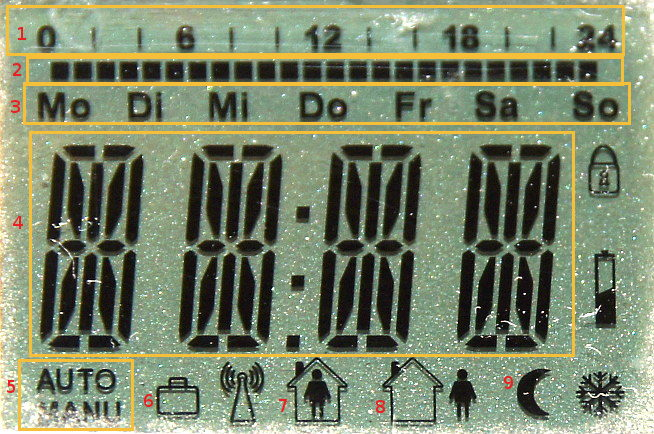
\includegraphics[width=0.7\linewidth]{LCD.jpg}
\caption{Elemente des LC-Displays}
\label{fig:LCD}
\end{figure}

Im Einzelnen handelt es sich dabei:

\begin{enumerate}
%1
\item \textbf{Stundenanzeige}\\ Diese Anzeige bezeichnet grob die
  Stunden des darunterliegenden Anzeigebalkens.  Die Stundenanzeige
  wird beim Start der Firmware aktiviert und dient daher als
  Ein\-schalt\-anzeige.
%2
\item \textbf{Anzeigebalken}\\ Der Anzeigebalken beschreibt im
  Automatikmodus bzw. während der Programmiermenüs für den
  Automatikmodus die Stunden des Tages, während derer die "`zu
  Hause"'-Temperatur aktiv ist.  Ein Kästchen entspricht einer Stunde.
%3
\item \textbf{Wochentagsanzeige}\\ In dieser Zeile wird der Wochentag
  angezeigt.  Im Normalzustand ist dies der aktuelle Wochentag gemäß
  der eingestellten Uhr, in den Programmierfunktionen wird dabei der
  Tag oder die Tage angezeigt, für den die Programmierung gerade
  erfolgt bzw. beim Urlaubs-Menü der Wochentag, der gerade als Ende
  des Urlaubs gewählt ist.
%4
\item \textbf{Hauptanzeige}\\ Hier werden im Normalzustand abwechselnd
  die aktuelle Uhrzeit und die letzte gemessene Temperatur angezeigt.
  Während der Menüfunktionen wird dort ein entsprechender Menütext
  angezeigt oder der aktuell eingestellte Wert.
%5
\item \textbf{Anzeige des Betriebsmodus}\\ Das Wort \texttt{MANU} wird
  angezeigt, wenn die Temperaturregelung gemäß dem manuell eingestellten
  Wert erfolgt.  Das Wort \texttt{AUTO} wird angezeigt, wenn das
  Temperaturprofil dem zuvor programmierten Zeitverlauf folgt.
%6
\item \textbf{Urlaubs-Symbol}\\ Wenn dieses Symbol angezeigt wird, dann
  ist derzeit eine Urlaubsfunktion aktiv.
%7
\item \textbf{"`zu Hause"'}\\ Wenn dieses Symbol angezeigt wird, dann
  folgt die Solltemperatur dem Wert für "`zu Hause"'.
%8
\item \textbf{"`außer Haus"'}\\ Wenn dieses Symbol angezeigt wird, dann
  folgt die Solltemperatur dem Wert für "`außer Haus"'.
%9
\item \textbf{"`Nacht"'}\\ Wenn dieses Symbol angezeigt wird, dann folgt
  die Solltemperatur dem Wert für "`Nachtbetrieb"'.

\end{enumerate}

\subsection {
  Tasten und Stell-Rad
}

Der Tastenblock des \SC{} besteht aus drei Tasten:

\begin{itemize}
\item \textbf{\texttt{MENU}}\\ Diese Taste schaltet den Menü-Modus ein oder aus.
\item \textbf{\texttt{OK}}\\ Diese Taste bestätigt im Menü-Modus eine bestimmte
  Einstellung oder Funktion.
\item \textbf{Uhr}\\ Diese Taste hat derzeit keine Funktion.  Die Uhrzeit wird
  in der Standard-Darstellung abwechselnd mit der Ist-Temperatur in der
  Hauptanzeige (Nr. 4 in Abbildung \ref{fig:LCD}) angezeigt.
\end{itemize}

Das Stell-Rad unter den Tasten erlaubt es, bestimmte Einstellungen zu
ändern oder durch die Menüs hindurch zu schalten.

Im Grundzustand wird durch dieses Rad die aktuelle Soll-Temperatur
der Regelung geändert.  Diese Änderung kann sowohl im manuellen als
auch im Automatikmodus (siehe Abschnitt \ref{sec:modi}) vorgenommen
werden.  Im Automatikmodus ist die Änderung jedoch nur so lange
wirksam, bis die aktuelle Phase im Temperaturprofil durch eine
andere Phase abgelöst wird.

\section {
  Beschreibung der Software
}

\subsection {
  Inbetriebnahme
}

Die Inbetriebnahme erfolgt durch Einlegen von 2 Batterien LR6 in das
Batteriefach.  Im Display erscheinen nach links wandernde kleine
Pfeile, die andeuten, dass der Stellmotor das Ventil maximal öffnet.
Anschließend blinkt der Text \texttt{INST OK}.  In diesem Zustand sollte
das Ventil auf den Heizkörper aufgesteckt werden.

Danach wird die \texttt{OK}-Taste betätigt, und die Firmware führt eine
Erstkalibrierung des Ventilwegs durch.

Danach sollte sinnvollerweise noch das aktuelle Datum sowie die
Uhrzeit eingetragen werden, siehe Abschnitt \ref{menu:zeit}.

Das \SC{} befindet sich danach im manuellen Betriebsmodus.

\subsection {
  Betriebsmodi: \texttt{MANU} vs. \texttt{AUTO}\label{sec:modi}
}

Im manuellen Modus regelt die Regelung auf die eingestellte Solltemperatur.
Die Solltemperatur lässt sich mit dem Einstellrädchen ändern.  Die
Änderung wird sofort wirksam; nach einigen Sekunden geht die Anzeige
wieder in ihren Wechsel zwischen Ist-Temperatur und Uhrzeit zurück.

Im Automatikmodus wird die Solltemperatur für die Regelung bei jedem
Übergang zwischen den einzelnen Zuständen ("`im Haus"', "`außer Haus"'
und "`Nacht"') an die voreingestellten Werte angepasst.  Der Sollwert
kann danach wie im manuellen Modus mit dem Stell-Rad noch geändert
werden; in diesem Falle bleibt er bis zum nächsten Übergang auf einen
neuen Zustand erhalten.

Für die Benutzung des Automatikmodus ist es notwendig, vorher das
Temperaturprofil zu programmieren (Abschnitt \ref{menu:prog} und
Abschnitt \ref{menu:temp}) sowie die Uhr einzustellen (Abschnitt
\ref{menu:zeit}).

\subsection {
  Menüführung
}

Durch Betätigen der Taste \texttt{MENU} wechselt man in den
Menü-Modus.  Durch Drehen des Stell-Rads durchläuft man anschließend
die Menüs der Hauptebene.  Die Auswahl eines Menüs daraus erfolgt
durch Betätigen der Taste \texttt{OK}.  Einzelne Menüs haben danach
weitere Untermenüs, zu denen ebenfalls durch die Taste \texttt{OK}
weitergeschaltet wird.  Innerhalb des Menüs lässt sich der aktuelle
Wert durch Drehen des Stell-Rads verändern.

Durch erneutes Betätigen der Taste \texttt{MENU} gelangt man aus dem
Menü-Modus stets zurück in den Standard-Modus (Anzeige von
Ist-Temperatur und Uhrzeit).

Die Menüpunkte der obersten Ebene werden im Folgenden beschrieben.

\subsubsection {
  Menü \texttt{MODE}
}

In diesem Menü wird zwischen manueller Betriebsart (Anzeige
\texttt{MANU}) und automatischer Betriebsart (Anzeige \texttt{AUTO})
umgeschaltet.  Beim Drücken der Taste \texttt{OK} wird die Betriebsart
entsprechend gewechselt.  Die Anzeige Nr. 5 in Abbildung \ref{fig:LCD} zeigt die
aktuell wirksame Betriebsart an.  Beim Wechsel auf Automatik-Modus
wird anschließend die Soll-Temperatur entsprechend dem aktuellen Tag
und Uhrzeit gemäß Temperaturprofil aktiviert.  Beim Wechsel auf
manuellen Modus bleibt die zuletzt wirksam gewesene Soll-Temperatur
eingestellt.

\subsubsection {
  Menü \texttt{PROG}\label{menu:prog}
}

In diesem Menü erfolgt die Programmierung der Temperaturprofile für
den Automatikmodus.

Die Temperaturprofile werden für jeden Tag separat gespeichert.  Über
die Menüpunkte \texttt{TAG1} bis \texttt{TAG7} lassen sich die Profile
von Montag bis Sonntag separat programmieren.  Außerdem gibt es noch
die Option, Sammelprofile für Montag bis Freitag (\texttt{T1-5}),
Montag bis Samstag (\texttt{T1-6}), die gesamte Woche (\texttt{T1-7})
oder das Wochenende (\texttt{T6-7}) festzulegen.  In diesem Falle
werden nach Abschluss der Programmierung des jeweiligen Sammelprofils
die Profile der betreffenden Tage entsprechend aktualisiert.  Dadurch
lassen sich anschließend diese Sammelvorgaben noch für einzelne Tage
überarbeiten, wenn gewünscht.

Alle programmierten Profile werden in einem nichtflüchtigen
Speicherbereich abgelegt, sodass sie auch nach einem Batteriewechsel
noch vorhanden sind.  Vollständig gelöscht werden können sie nur über
das \texttt{RES}-Menü, siehe Abschnitt \ref{menu:res}.

Für jeden Tag enthält das Profil vier Zeitpaare für den Wechsel
zwischen "`zu Hause"'- und "`außer Haus"'-Temperatur, sowie
abschließend eine Uhrzeit, ab der die "`Nacht"'-Temperatur
wirksam wird.  Diese bleibt aktiv, bis am nächsten Tag die erste
"`zu Hause"'-Zeit heran ist.

Alle Zeiten lassen sich in 10-Minuten-Schritten einstellen.  Wenn ein
Zeitpaar für das Einschalten (\texttt{STRT}) und Ausschalten
(\texttt{ENDE}) der "`zu Hause"'-Temperatur gleiche Zeiten enthält
(bspw. die Voreinstellung \texttt{00:00}), so wird es nicht benutzt.

\subsubsection {
  Menü \texttt{TEMP}\label{menu:temp}
}

In diesem Menü erfolgt die Festlegung der Solltemperaturen für die
einzelnen Zeitfenster des Automatikmodus.

In den Untermenüs werden der Reihe nach die Temperatur für "`zu
Hause"', "`außer Haus"' und "`Nacht"' in Schritten von 0,5~K
festgelegt.  Dabei wird das jeweilige Symbol (Nr. 7, 8 und 9
in Abbildung \ref{fig:LCD}) eingeblendet.  Die Festlegung des
ausgewählten Wertes erfolgt mit der \texttt{OK}-Taste, danach
wird zum nächsten Wert weitergeschaltet.

Nachdem alle drei Werte festgelegt worden sind, werden sie im
nichtflüchtigen Speicher hinterlegt, sodass sie auch nach einem
Batteriewechsel wirksam bleiben.

\subsubsection {
  Menü \texttt{ZEIT}\label{menu:zeit}
}

In diesem Menü erfolgt die Einstellung von Datum und Uhrzeit.

Eine korrekte Einstellung der geräteinternen Uhr ist wichtig, wenn
der Automatikmodus benutzt werden soll.

Die Einstellung erfolgt, indem der Reihe nach das Jahr, der Monat,
der Tag, Stunde und Minute gewählt werden.  Der entsprechende Wert
wird anschließend mit der \texttt{OK}-Taste bestätigt, und die
Einstellung springt zum nächsten Wert.  Der jeweils veränderliche
Wert wird dabei blinkend dargstellt.

Beim Batteriewechsel wird die aktuelle Zeiteinstellung in einem
nichtflüchtigen Speicher (EEPROM) im Gerät zwischengespeichert.  Nach
dem Einsetzen neuer Batterien läuft sie mit dieser gespeicherten Zeit
erneut an.  Natürlich kann die Uhr nicht weiterzählen, während keine
Batterien im Gerät sind, es gehen also einige Sekunden dabei
verloren.

\subsubsection {
  Menü \texttt{FENS}
}

Dieses Menü ist für die Funktion "`Fenster offen"' vorgesehen.

Diese Funktion ist derzeit nicht implementiert.

\subsubsection {
  Menü \texttt{RES}\label{menu:res}
}

Dieses Menü dient dem vollständigen Rücksetzen aller gespeicherten
Daten (Temperaturprofil, Ventilstellung und -stellweg).  Es sollte nur
benutzt werden, wenn das \SC{} von einem Heizkörper zu einem anderen
umgesetzt wird.

Im Anschluss an die Bestätigung des \texttt{OK}-Punktes startet die
Firmware komplett von vorn, beginnend mit einer Rekalibrierung, um
sich auf den neuen Heizkörper einstellen zu können.

\subsubsection {
  Menü \texttt{ADAP}
}

Durch Bestätigung dieses Menüs mit der \texttt{OK}-Taste erfolgt
eine Rekalibrierung der Ventilstellung.  Das Ventil wird zuerst
vollständig geöffnet, es erscheint die Ausschrift \texttt{INST OK},
und nach Drücken der \texttt{OK}-Taste werden die Positionen des
Heizkörperventils für "`offen"' und "`geschlossen"' erfasst.

Danach wird zum normalen Regel-Modus zurückgekehrt.

Der Aufruf dieses Schritts ist notwendig, falls sich zeigt, dass im
laufenden Betrieb die Heizung auch dann warm bleibt, obwohl die
Temperatur hoch genug ist und das Ventil eigentlich vollständig
geschlossen sein sollte.  Dies kann mit der in Abschnitt
\ref{menu:dbg-posi} beschriebenen Testfunktion verifiziert werden.
Wenn dort \texttt{POSI} als 0 angezeigt wird, das Ventil aber dennoch
offenbar leicht geöffnet ist (Heizung bleibt auch nach längerer
Wartezeit warm), dann stimmt die interne Erfassung der Ventilposition
nicht mehr mit der Realität überein, und es sollte eine Rekalibrierung
gestartet werden.

\subsubsection {
  Menü \texttt{URLA}
}

In diesem Menü wird die Urlaubs-Funktion aktiviert.

Durch Drehen des Stell-Rads kann das Datum für das Ende des Urlaubs
eingestellt werden, beginnend beim Jahr.  Die Anzeige wechselt dabei
jeweils zwischen \texttt{URLA} (bzw. Teilen davon) und dem aktuellen
Wert.

Die Urlaubsfunktion wird aktiv, sowie alle drei Werte (Jahr, Monat
und Tag) eingestellt worden sind.  Während des Einstellens wird
die Anzeige für den Wochentag (Nr. 3 in Abbildung \ref{fig:LCD}) entsprechend
des gewählten Datums für das Urlaubsende aktualisiert.

Beim Erreichen des eingestellten Datums (Mitternacht) wird die
Urlaubsfunktion anschließend automatisch gelöscht und das reguläre
Temperaturprofil reaktiviert.

Während des Urlaubs-Modus wird das normale Temperaturprofil bewertet
wie sonst, aber statt der "`zu Hause"'-Temperatur wird die "`außer
Haus"'-Temperatur als Sollwert benutzt.  Die Nachttemperatur
verbleibt dagegen in gleicher Weise wie im normalen Automatik-Modus.

Als Hinweis auf die aktive Urlaubs-Funktion wird das Symbol Nr. 6
in Abbildung \ref{fig:LCD} angezeigt.

\subsubsection {
  Menü \texttt{INST}
}

Durch Aktivieren dieses Menüpunktes öffnet sich das Ventil
vollständig, sodass man es ohne Kraftaufwand erneut auf
den Heizkörper aufstecken kann.

Durch anschließendes Betätigen der \texttt{OK}-Taste schließt
es sich wieder.

\subsubsection {
  Menü \texttt{OFFS}
}

In diesem Menü lässt sich ein Korrekturfaktor zur internen
Temperaturmessung festlegen.  Die Einstellung erfolgt in Schritten zu
0,5~K.  Der eingestellte Wert wird zur gemessenen Temperatur addiert;
ist er negativ, wird die Temperatur also um den Betrag dieses Werts
reduziert.

Die Anzeige der Ist-Temperatur im regulären Anzeigemodus
berücksichtigt diesen Wert.

\subsubsection {
  Menü \texttt{DBUG}
}

In diesem Untermenü können einzelne interne Parameter der Firmware
abgefragt werden, um die Funktion zu überprüfen bzw. Fehler eingrenzen
zu können.  Im Einzelnen sind dies:

\begin{description}
\item[\texttt{FIRM}] Versionsnummer der Firmware
\item[\texttt{FUZZ}] Gegenwärtiger Zustand des Regelalgorithmus,
  bestehend aus zwei Buchstaben.

  Erster Buchstabe, Zustand:
  \begin{description}
  \item[\texttt{O}] Temperatur im Sollbereich ("`OK"')
  \item[\texttt{W}] Temperatur zu warm
  \item[\texttt{H}] Temperatur zu heiß
  \item[\texttt{C}] Temperatur zu kühl ("`Cool"')
  \item[\texttt{D}] Temperatur zu kalt ("`Col\emph{d}"')
  \item[\texttt{A}] Temperatur viel zu heiß ("`Above"')
  \item[\texttt{B}] Temperatur viel zu kalt ("`Below"')
  \end{description}

  Zweiter Buchstabe, Tendenz:
  \begin{description}
  \item[\texttt{S}] Temperatur gleichbleibend ("`Static"')
  \item[\texttt{R}] Temperatur steigt ("`Rising"')
  \item[\texttt{F}] Temperatur fällt
  \end{description}
\item[\texttt{POSI}] Aktuelle Ventilposition, 0 = geschlossen\label{menu:dbg-posi}
\item[\texttt{VTOP}] Position für "`Ventil ganz geöffnet"'
\item[\texttt{RWAY}] Anzahl der Schritte in der letzten Regel-Aktion; positive
  Werte bezeichnen dabei ein Öffnen des Ventils um diese Anzahl, negative
  Werte ein Schließen.
\item[\texttt{$\Delta$TMP}] Letzte und vorletzte Temperaturdifferenz, hexadezimal
\end{description}

\section {
  Danksagung
}

Besonderer Dank gilt den zahlreichen Mitwirkenden aus dem Forum von
\texttt{http://www.mikrocontroller.net/} für ihre Analyse und
Dokumentation der Hardware des \SC, sowie ganz speziell Knut Ballhause
für seine Version der Firmware, die durch die vorliegende
Implementierung anschließend erweitert und ergänzt worden sind.

Ohne all diese Vorarbeit wäre die vorliegende Implementierung nicht
mit vertretbarem Aufwand möglich gewesen.

\section {
  Urheberrecht, Lizenz
}

Die Alternativ-Firmware wurde von Knut Ballhause als \emph{Public Domain}
deklariert \footnote{\texttt{https://creativecommons.org/publicdomain/zero/1.0/}}, die
Umarbeitung von Assembler in C sowie die darauf aufbauenden Ergänzungen
durch Jörg Wunsch ebenfalls.

Diese Dokumentation wurde von Jörg Wunsch geschrieben, sie steht unter
der Lizenz CC-BY\footnote{\texttt{https://creativecommons.org/licenses/by/2.0/}}.

\end {document}

